%&latex
\documentclass[12pt]{article}
\usepackage{amsthm,amsmath}
\usepackage{graphicx,psfrag,epsf}
\usepackage{enumerate}
\usepackage{natbib}
\usepackage{url} % not crucial - just used below for the URL
\usepackage{amsthm,amsmath}
\usepackage[utf8]{inputenc}

%\pdfminorversion=4
% NOTE: To produce blinded version, replace "0" with "1" below.
\newcommand{\blind}{0}

% DON'T change margins - should be 1 inch all around.
\addtolength{\oddsidemargin}{-.5in}%
\addtolength{\evensidemargin}{-.5in}%
\addtolength{\textwidth}{1in}%
\addtolength{\textheight}{1.3in}%
\addtolength{\topmargin}{-.8in}%


\begin{document}

%\bibliographystyle{natbib}
%\bibliographystyle{bmc-mathphys}
\bibliographystyle{agsm}

\def\spacingset#1{\renewcommand{\baselinestretch}%
{#1}\small\normalsize} \spacingset{1}


%%%%%%%%%%%%%%%%%%%%%%%%%%%%%%%%%%%%%%%%%%%%%%%%%%%%%%%%%%%%%%%%%%%%%%%%%%%%%%

\if0\blind
{
  \title{\bf Teaching analysis reproducibility with accessibility: Enriching secondary documentation to support skill level diversity of users.}
  \author{Luna L. Sanchez Reyes\thanks{
    The authors gratefully acknowledge ``Sustaining the Open Tree of Life``, NSF ABI No. 1759838, and ABI No. 1759846.}\hspace{.2cm}\\
    School of Natural Sciences, University of California, Merced\\
    and \\
    Emily Jane McTavish \\
    School of Natural Sciences, University of California, Merced}
  \maketitle
} \fi

\if1\blind
{
  \bigskip
  \bigskip
  \bigskip
  \begin{center}
    {\LARGE\bf Teaching analysis reproducibility with accessibility: Enriching secondary documentation to support skill level diversity of users.}
\end{center}
  \medskip
} \fi

\bigskip
\begin{abstract}
Research reproducibility is essential for scientific development. Yet, rates of reproducibility
are low, especially in the natural sciences. As increasingly more research is relying on
computing tools and software, efforts for improving
reproducibility rates have focused on digital availability of research workflows
as computer code, as well as raw and processed data in computer readable form.
However, making research products digitally available does not
necessarily ensures that
they can be easily reached by the majority of a target user base, let alone the general population,
making them effectively inaccessible, counteracting availability, and hindering reproducibility.
Thus, accessibility of research products is a key aspect for the long term improvement
of reproducibility rates.
Using an example within evolutionary biology, we identify inclusivity barriers to accessibility,
% accessibility typically refers to addressing differences in abilities (visual, hearing, cognitive).
research products in the natural sciences:
%% list the barriers
use of highly specialized computing jargon and programming techniques; high cognitive load,
unspecified, unclear or lengthy goals; content-focused descriptions instead of user-focused;
inflexible learning environment; unapproachable (cold or intimidating) language;
and little to no diversity of representation of information.

Then, we propose a set of principles to improve accessibility of code and data,
and illustrate their application in a set of teaching materials for evolutionary biology that we put
to work in the field.
Finally, we elaborate on the general application of these principles for
documenting scientific workflows, to provide present learners
and future researchers with tools for successful scientific reproducibility.
%> ** add a sentence on implications for teaching reproducibility


%% Projects that address availability of code and data in the natural sciences
%% have focused on producing documentation that describes the nature and usage of the
%% resources.
%% However, it is often written using highly specialized language that is largely
%% inaccessible for the average target user. Additionally, baseline
%% computational knowledge and skills required to access scientific results are often
%% not found among potential users, and keep on increasing.

%% **Introduce OpenTree in abstract??




\end{abstract}

\noindent%
{\it Keywords:}  open science, R, phylogenetics, Open Tree of Life
\vfill

\newpage
\spacingset{1.45} % DON'T change the spacing!
\section*{Introduction}
\label{sec:intro}

Research reproducibility --the extent to which consistent results are obtained when
a scientific experiment or research workflow is repeated \citep{repdef2021}--
is a key aspect of the advancement
of science, as it constitutes a minimum standard that allows understanding research products
(e.g., methods, data, analysis, results, etc.)
to determine their reliability and generality, and eventually build up scientific
knowledge and applications based on those products
\citep{king1995replication, peng2011reproducible, powers2019open}.
In the natural sciences, rates of reproducibility are low \citep{ioannidis2005most, prinz2011believe},
which has elicited concerns about a crisis in the field \citep{baker2016reproducibility}.
%%% The scientific community has united to incentivize cultural changes that will improve
%%% reproducibility rates long term, such as transparency, availability, and workflow
%%% automatization, to name a few \citep{peng2015reproducibility}.
In response, the scientific community has been developing new principles and standards to incentivize
cultural changes in an effort to improve long term reproducibility rates in the natural sciences
\citep{peng2015reproducibility, wilkinson2016fair}.
A standard for reproducibility that has received much attention is scientific availability, which
we define as a property denoting that a research product can be reached (acquired, copied, analyzed,
processed and/or reused) at no financial, legal or technical cost \citep{arnold2019turing},
and without geographic, demographic, social or temporal barriers for the population \citep{fecher2014open}.
In this paper, we argue that availability can not be fully achieved without accessibility (Box 1).

We recognize that the term accessibility is used in relation to various aspects of
the human experience. In relation to digital resources, these aspects have been broadly
categorized in four axis: perception, operability, understanding and robustness \citep{chisholm2001web, caldwell2008web}
% (visual, motor, auditory, cognitive, social, psychological, educational, etc.).
Some forms of accessibility do not support automatization nor scalability.
For example, Graphical User Interfaces (GUIs) are accessible, but not scalable and rarely automatizable.


we focus on X types of accessibility

% not all types of accessibility support reproducibility
% while accessibility is key to support availability, and availability is ket for reproducibility,
% some forms of accessibility do not support reproducibility.

We identify factors that have particularly affected accessibility in
the natural sciences, and ways the scientific community can address them to create reproducible
research workflows. These principles can be generalized and integrated
into the undergraduate and graduate school STEM curriculum, either for courses specialized
in reproducibility or within other subject areas, as a necessary component of
successful and impactful science.

% ** describe/introduce reproducibility curriculum here


\bigskip
\bigskip

\noindent\fbox{%
    \parbox{\textwidth}{%
    \textbf{Box 1. The role of accessibility in improving reproducibility.}
      % Availability is defined as the fact or possibility that something can be bought,
      % used, or reached by someone \citep{availability2022cambridge}.
      % Accessibility is defined as "the fact of being able to be reached or obtained easily"
      % \citep{accessibility2022cambridge}
      Availability and accessibility are conceptually accepted as synonyms for ``the fact
      of being able to be reached" \citep{available-accessible2022cambridge}.
      However, accessibility's definition goes further and describes it as the
      ``fact of being able to be reached \textbf{easily}" \citep{accessibility2022cambridge}.
      A secondary definition of accessibility elaborates more on this: ``the quality
      of being \textbf{easy to understand}''.
      % Yet, in practice, availability does not imply accessibility.

      What we realize from these definitions is that, in practice, something might
      be available but not necessarily accessible,
      hindering the realization of availability.
      To illustrate the practical difference between availability and accessibility we
      will use an allegory that goes like this:

      ** Change marshmallow story to cake

      ** Explain different types of barriers to accessibility within the example, then within science

      ** Explain why we focus on psychological/social/pedagogical barriers

      ** Gauging accessibility of a resource is tricky because it depends on an
      individual experience of what is in effect \textbf{easy} for someone.
      \textbf{Easy} is a subjective quality that fully depends on individual perceptions
      resulting from individual contexts.
      As a society we are moving towards validating and welcoming all human experiences.
      To improve accessibility levels in the natural sciences, it
      is important to account for the factors that are creating different experiences
      of what is \textbf{easy}.

      ** Now, explain different types of barriers to accessibility in science
      (Jessica: Maybe say that lack of accessibility can be due to a number of
      factors (physical, resources, economic), but one critical factor is the use
      of impenetrable expert language.)
    }%
}
\bigskip

\section*{An example from phylogenetics}
\label{sec:example}

To elaborate on our thesis,
%% we use a common scientific workflow in phylogenetics,
%% ** Jessica mentions that workflow is confusing as she thought it referred to the OpenTree
%% workflow, but we actually mean the more general workflow of reconstructing a phylogenetic tree.
%% She suggests something more general:
we choose an example from the research field of phylogenetics,
a discipline within evolutionary biology. Phylogenetics focuses
on investigating the history of shared ancestry of living organisms from biological data,
and represents
this evolutionary history in a diagram known as a phylogeny (Figure \ref{fig:tree}).
Phylogenies provide the
basis to study and understand all biological processes in an evolutionary context
\citep{dobzhansky1973nothing}. Hence,
% Given the importance of phylogenies for biological research,
it appears that improving reproducibility rates
in phylogenetics has the potential to positively impact research across the natural sciences.

***What other platforms provide resources for reproducibility in phylogenetics???

The Open Tree of Life project (OpenTree) has developed a computational platform that provides
digital availability of phylogenetic results from vetted, state-of-the-art research
in the field \citep{opentreeoflife2019synth}.
%% by creating a standardized database of phylogenetic data that is used to synthesize
%% a single phylogenetic tree encompassing all life
OpenTree's database, the Phylesystem \citep{mctavish2015phylesystem}, provides
usability of phylogenetic data by standardizing organism names across biological databases,
and supporting digital data obtention in a computer readable format.

While this is accessible through their Graphical User Interface,
It does not support reproducibility

Accessibility does not imply reproducibility

In order for something to be highly reproducible, it has to be largely accessible.


is programmatically
available free of cost to users through OpenTree's Application Programming Interface
(API) services \citep{opentreeAPIv3}.
Additionally, software packages written with open source, free of cost programming
languages commonly used in scientific research such as R and Python
\citep{baker2017scientific} have been developed as wrappers that have increased the availability
of OpenTree's API services, by making the OpenTree API functionalities more accessible
to a wider user audience \citep{michonneau2016rotl, mctavish2021opentree}.
Yet, the R and Python OpenTree API wrapper software packages have been mainly used
by computer-literate individuals
to seamlessly establish reproducible workflows to use and reuse expert phylogenetic
knowledge for biological research \citep{sanchez2019datelife, sanchez2021physcraper}
and education \citep{nguyen2020phylotastic, phylotasticedtools, galacticedtools}.
In the 5 years since its release, the R package wrapper for OpenTree \texttt{rotl}
has been cited by more than 190 biological research papers addressing various
topics \citep{googlerotl}.
Comparatively, other R packages for phylogenetics, such as \texttt{GGTREE}
and \texttt{mixOmics}, which were released one year after \texttt{rotl} have been
cited over a thousand times, which might indicate a delay \texttt{rotl}
adoption. Of course one potential explanation is that OpenTree services do not have
as wide an application as services provided by the afore mentioned R packages.
However, the
expressed enthusiasm (interest to use/inability to use the resource) by the target
 audience and larger community might point to a different issue.
%% We need a proper statistical distribution of citation numbers per year, to see
%% if rotl is an outlier or not.

While learners in the natural sciences have been engaging independently with R
and Python programming languages
as they represent two of the most widely used programming languages in the sciences
% for their fast and seamless statistics and data analysis environment
\citep{baker2017scientific}, computer programming is not traditionally
a core skill formally taught to biologists and naturalists
\citep{sayres2018bioinformatics, wright2019the, williams2019barriers}.
Moreover, the main usage of the OpenTree API services hints that tools intended to
improve availability and reproducibility come at a cost for the potential users:
 an increased required baseline computational knowledge and skillset
in the field.
As computers continue to play a larger role in most scientific disciplines \citep{piccolo2016tools},
higher baseline computational skills are required across all natural sciences.
% "Thus efforts to increase scientific reproducibility should consider the ubiquity of computers in research."
% In order for reproducible computational tools to be adopted for research, they
% need to be readily accessible for present and future researchers.
Thus, efforts to increase reproducibility rates in the natural sciences must consider
the specifics of scientific workflows that rely on usage of programming languages, such as
availability and accessibility of data and code \citep{peng2011reproducible, sandve2013ten, powers2019open}.
% However, the utility of data resources is limited by the technical challenges of accessing the data.
% In order to motivate reproducible research, that gap needs to be bridged.
% In this work we focus on improving accessibility of code examples and documentation.

We chose a phylogenetics workflow that relies on data and code from OpenTree to
identify the specific barriers to accessibility it presents.
Then, we design ways to overcome or diminish these barriers and apply them to
a series of tutorials and vignettes developed for the OpenTree project.
The tutorials are available at https://mctavishlab.github.io/R\_OpenTree\_tutorials/.

Finally, we generalize our findings to suggest a set of
principles that can be used as a guide to develop code and documentation materials
with increased accessibility, to improve availability and contribute to reproducibility.
Notably, these principles can be incorporated as learning goals into any syllabus for a
course or workshop on best practices for scientific reproducibility.
% In particular, we identify the necessity for documentation that is written down
% using language that is common to the target audience to facilitate examination,
% application, and adoption of code by the wider audience.

\begin{figure}
\begin{center}
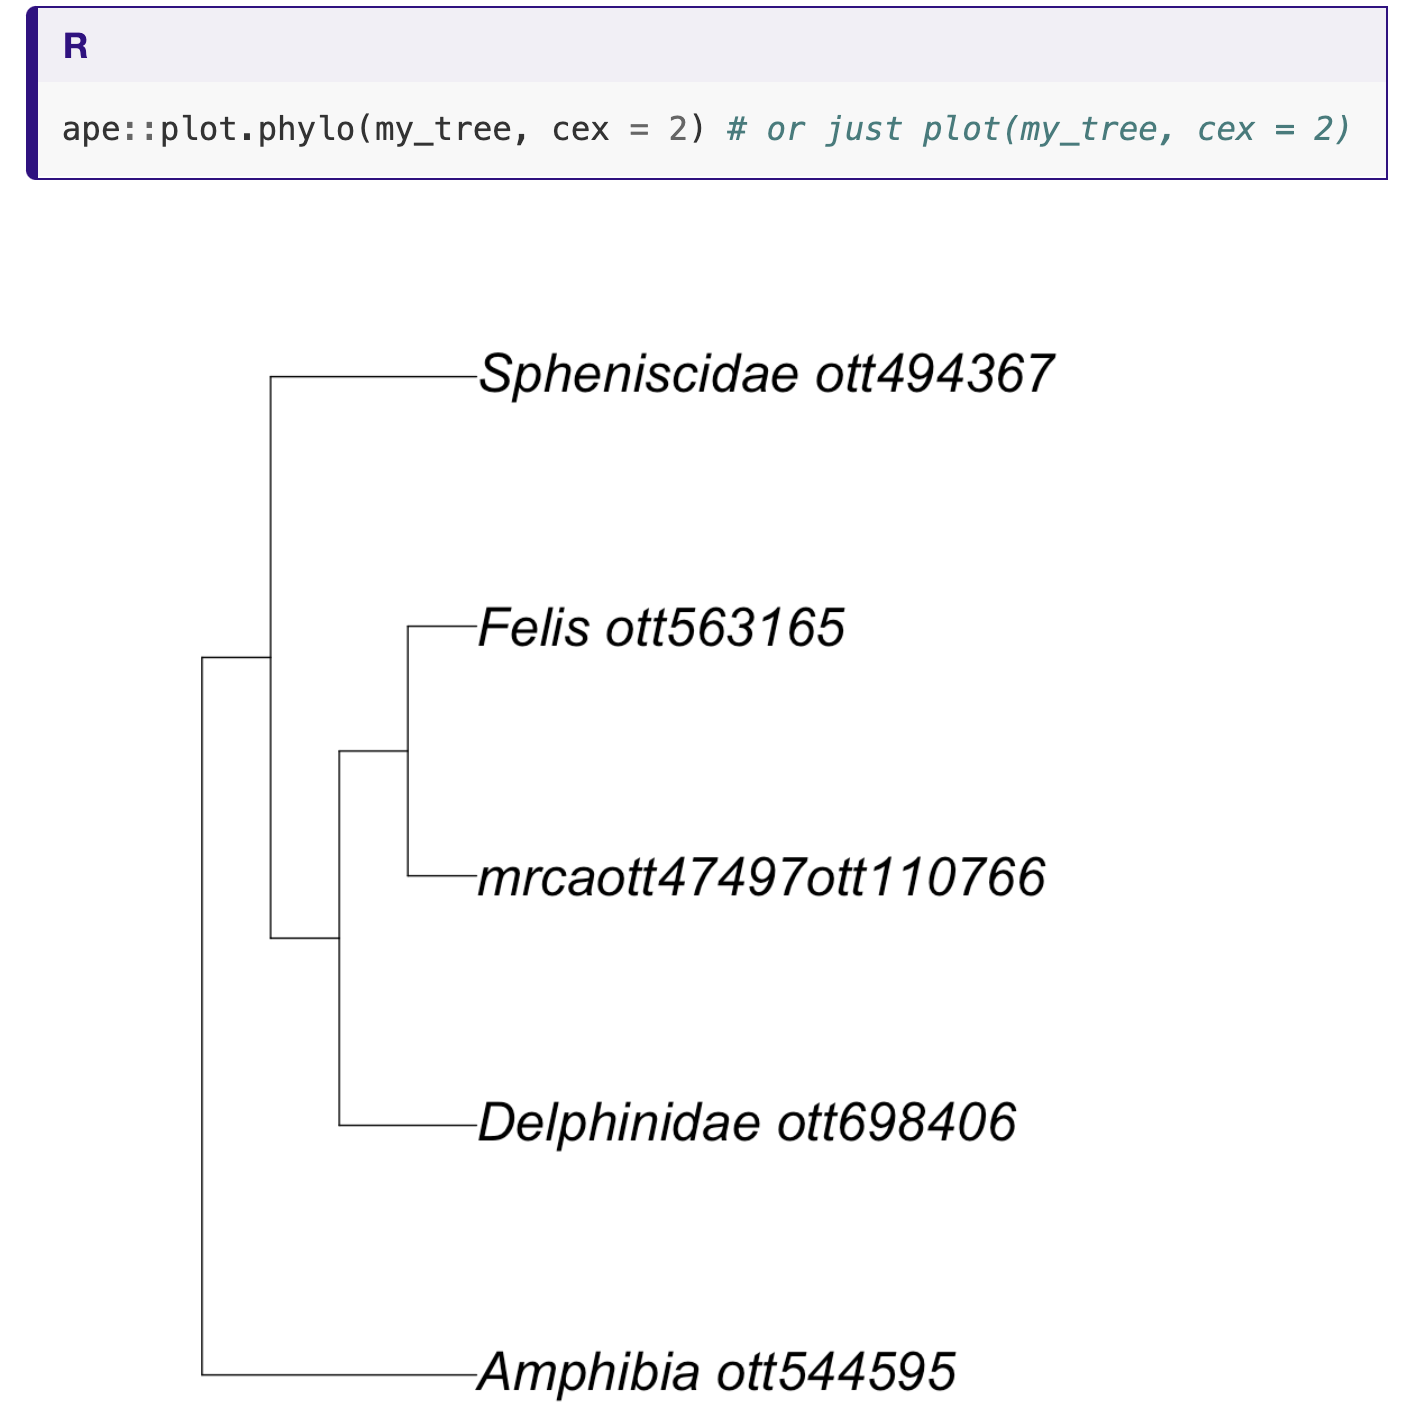
\includegraphics[width=3in]{fig-tree.png}
\end{center}
\caption{A phylogenetic tree from our tutorial website, extracted using OpenTree of Life tools and the rotl R package. \label{fig:tree}}
\end{figure}

\section*{Identifying hurdles to accessibility}
\label{sec:identifying}

Good primary documentation for code is thorough. It describes general usage of individual functions,
the components and variables a function can take, and it should be accompanied with
function usage examples on how to apply it \citep{karimzadeh2018top}.
As opposed to code, primary documentation is written in natural language (i.e.,
any known human language, e.g., English, Spanish, Chinese).
Primary documentation is viewed as a key element for success of a piece of code
\citep{karimzadeh2018top},
which might be why it is also usually written using highly specialized computational jargon (i.e., computationally specific concepts,
words, and phrases) as well as formal scientific language.
While this might be important for formal acceptance of the code by the scientific
and academic community, it often slows down or even
obstructs examination, application, and adoption of code by the general audience \citep{ball2017its}.

Vignettes and tutorials work as secondary pieces of documentation, that help to demonstrate
additional cases of individual function usage, and showcase function associations
that work for specific analysis workflows in more detail.
As secondary documentation has become more common practice and is more flexible
in its form and content, it constitutes an ideal canvas to develop, implement and
test principles that can overcome current barriers to code accessibility.

\section*{Addressing hurdles to accessibility: some principles}
\label{sec:addressing}

\subsubsection*{a. Literate programming: Demonstrate code usage with integrative examples}

%% I think I have three different points here:
%% internalizing knowledge is made easier with active learning practices: learn by doing!
%% literate programming allows learning by doing AND at the same time provides a story that connects the acquired knowledge to a real worl problem.
%% By definition, all languages are abstract. We learn them because we grow up with them and they have a direct application for our lives.
%% Programming languages are no different, however, we start learning those later in life and we do not use them as regularly, making it harder for us to learn them and use them.
Pedagogical research shows that active learning practices are one the most effective
ways to take on abstract subjects \citep{freeman2014active}.
Programming computer languages are quite abstract and learning them can be greatly
enhanced by applying an active learning strategy such as linking its usage to
a ``real world'' or ``human'' application \citep{felder2009active}.

A story-like narrative that links pieces of code together and invites learners
to try the code, can lead learners to remember what they are doing and
why they are doing it.
This ``literate programming'' paradigm \citep{knuth1984literate, fritzson2002mathmodelica}
makes code more approachable, as it integrates narratives with computer code in
the same document, supporting learners in actively following
the code usage, supporting memory and understanding \citep{piccolo2016tools}.

We propose that documents developed with ``literate programming'' can be made more
accessible by choosing narratives that are relatable to a more general audience.
An easy way to do this in biology is choosing as model organism a taxon that a
research group is more interested in studying. For the non-specialized user base,
a highly charismatic group such as dinosaurs will do the trick.


We examined available primary documentation for the package \texttt{rotl},
and designed a narrative that required the usage of as many functions as possible.
We demonstrate code applications that are commonly requested by OpenTree users,
but that are not demonstrated in the primary documentation of the R package.
By framing the function workflow using highly requested uses, the documentation acquires a
narrative arc that is easier to follow and remember by users. This can also facilitate
the application of code to other use cases in biology of interest for the users.

%% Maybe Figure!! For the tutorial demonstrated here, we used the commonly requested
%% use case of obtaining
%% a phylogenetic tree for all lineages within a specific taxonomic rank.

\subsubsection*{b. Demonstrate errors and warnings thoroughly}

A practice that has become more and more widespread in programming-language pedagogical practices
is the use of typos and mistakes to normalize them for learners, and show them how
to solve them when they are outside the classroom \citep{shannon2015live}.
Yet, this is rarely done on written pedagogical materials.
Primary documentation focuses on demonstrating usage function with examples that
work seamlessly, without errors. We argue that the opposite is needed to support
adoption of reproducible workflows and support long term independence in learners
\citep{gaspar2007restoring}.
We demonstrate examples that do not work
as expected and exemplify ways to address them (Figure \ref{fig:error}).

We identify inputs that would give
a wide range of warnings and errors, focusing on demonstrating these cases. This
helps users to not be afraid of errors and warnings, but instead to use them to
their advantage.
We also identify effects of warnings and errors downstream of the workflow.

We identify ways to evaluate inputs to know if they will produce an error, and design
alternatives on what to do when faced with an error or warning, and demonstrate
these alternatives.
One of the most essential skills in programming is interpreting and moving forward
from errors.
Many finely honed tutorials do not trigger errors, which precludes helping students
to develop the tools to understand and address errors when they do encounter them,
as they inevitably will.
In our tutorial, we focus on explaining the meaning and downstream of warnings and errors, and
 showcase ways to detect them before they are triggered (i.e., before using an input
  that would elicit a warning or error). This has two pedagogical benefits:
1) it provides users/students with the means to troubleshoot their own warnings and errors, and
2) it allows users/students to understand with more depth what the function is doing.

% We designed ways to access the different elements of the outputs.

\begin{figure}
\begin{center}
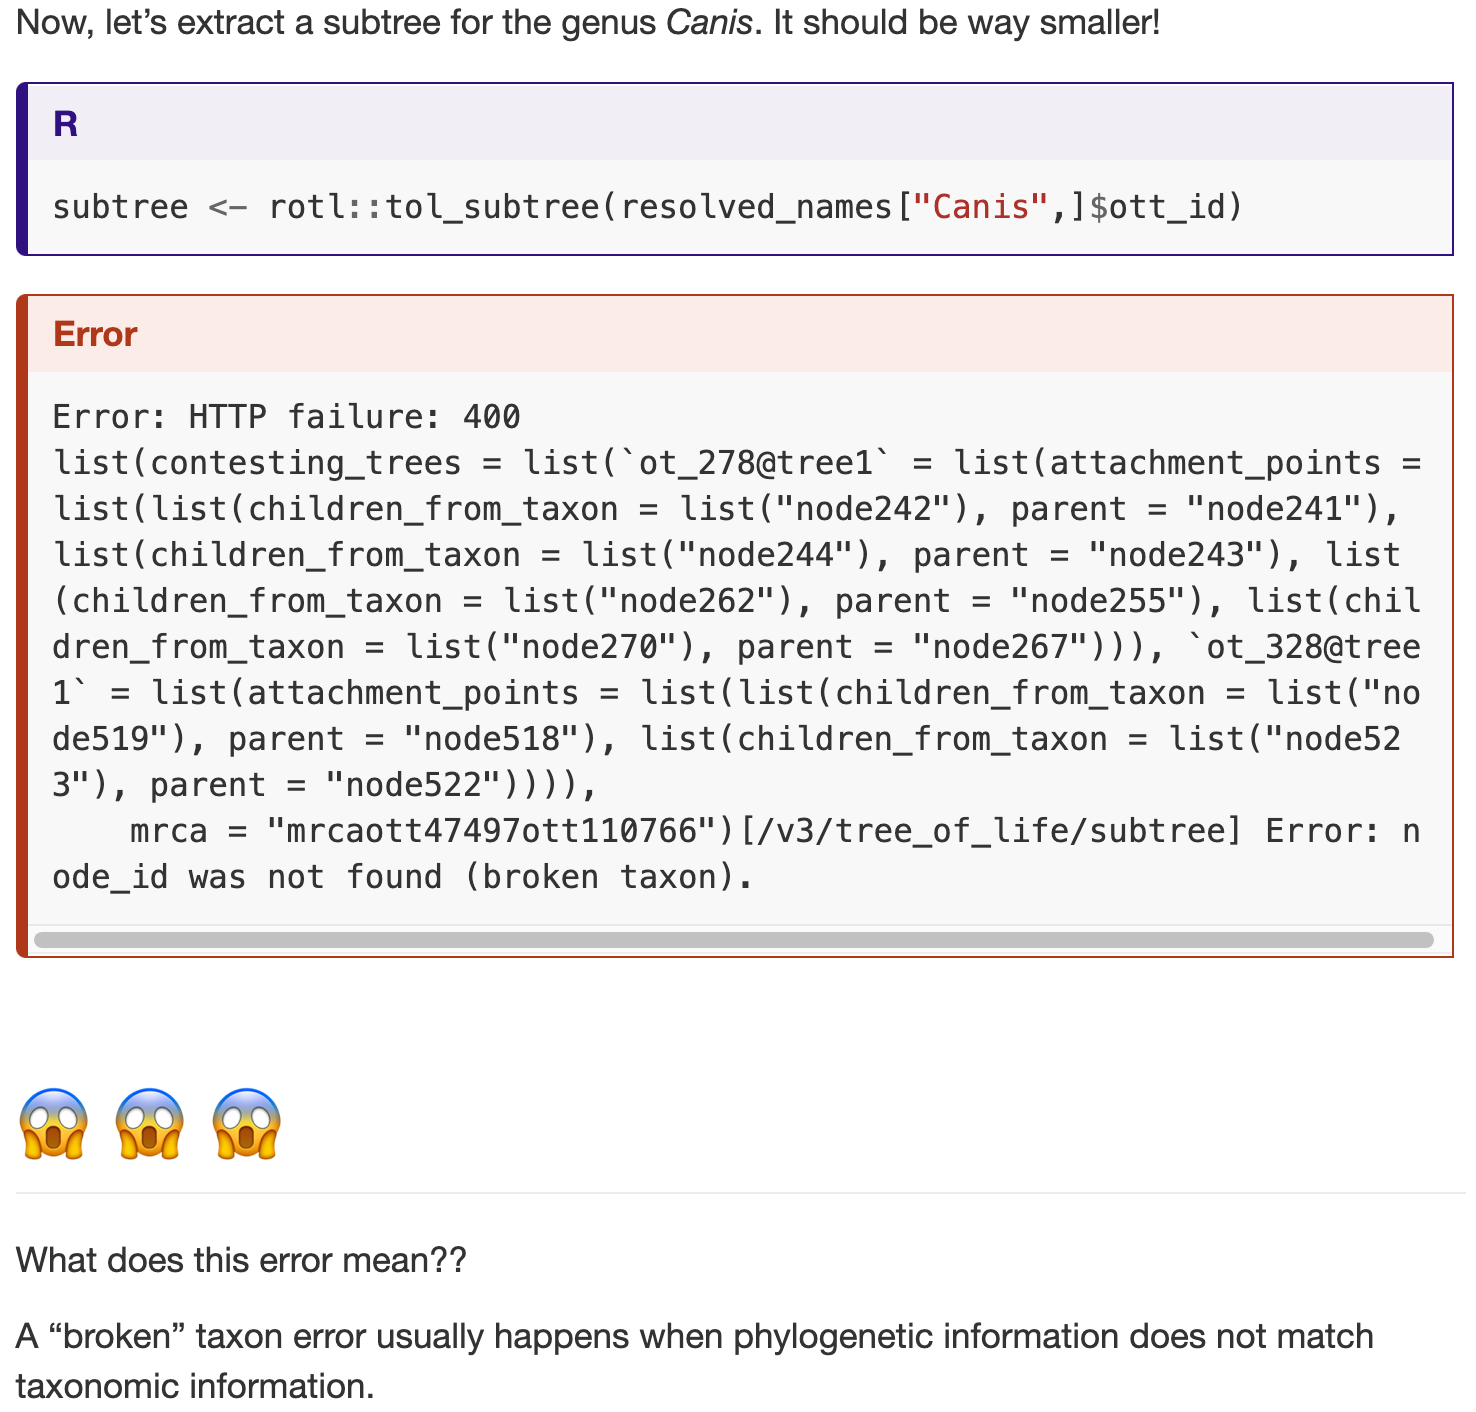
\includegraphics[width=3in]{fig-error.png}
\end{center}
\caption{Snapshot of a section of the tutorial website, where we demonstrate a common error. \label{fig:error}}
\end{figure}

\subsubsection*{c. Avoid jargon and expert language}

Besides avoiding formal language, and incorporating elements of pop culture, such as picture
character icons known as ``emojis``, to make the language more familiar to a
broader target audience (see Figure \ref{fig:error}), we made an effort to specifically
complement the primary documentation by identifying
computational concepts that were assumed or were not explained in depth.
We vetted the tutorials through feedback from workshop participants as well as individual users.
We choose examples that are charismatic for the audience.
For example, when we presented the tutorial for a team specialized in Amphibians,
we tailored the examples using frogs and their allies.


\subsubsection*{d. Make it stable through time}

We published the tutorials on a public, free license, free of cost, and free for
use and reuse repository and persistent website \citep{RopentreeTutorials}.
The tutorial is available for the users to go back to any time they need it,
and to be passed on to other users (Figure \ref{fig:schedule}).

\begin{figure}
\begin{center}
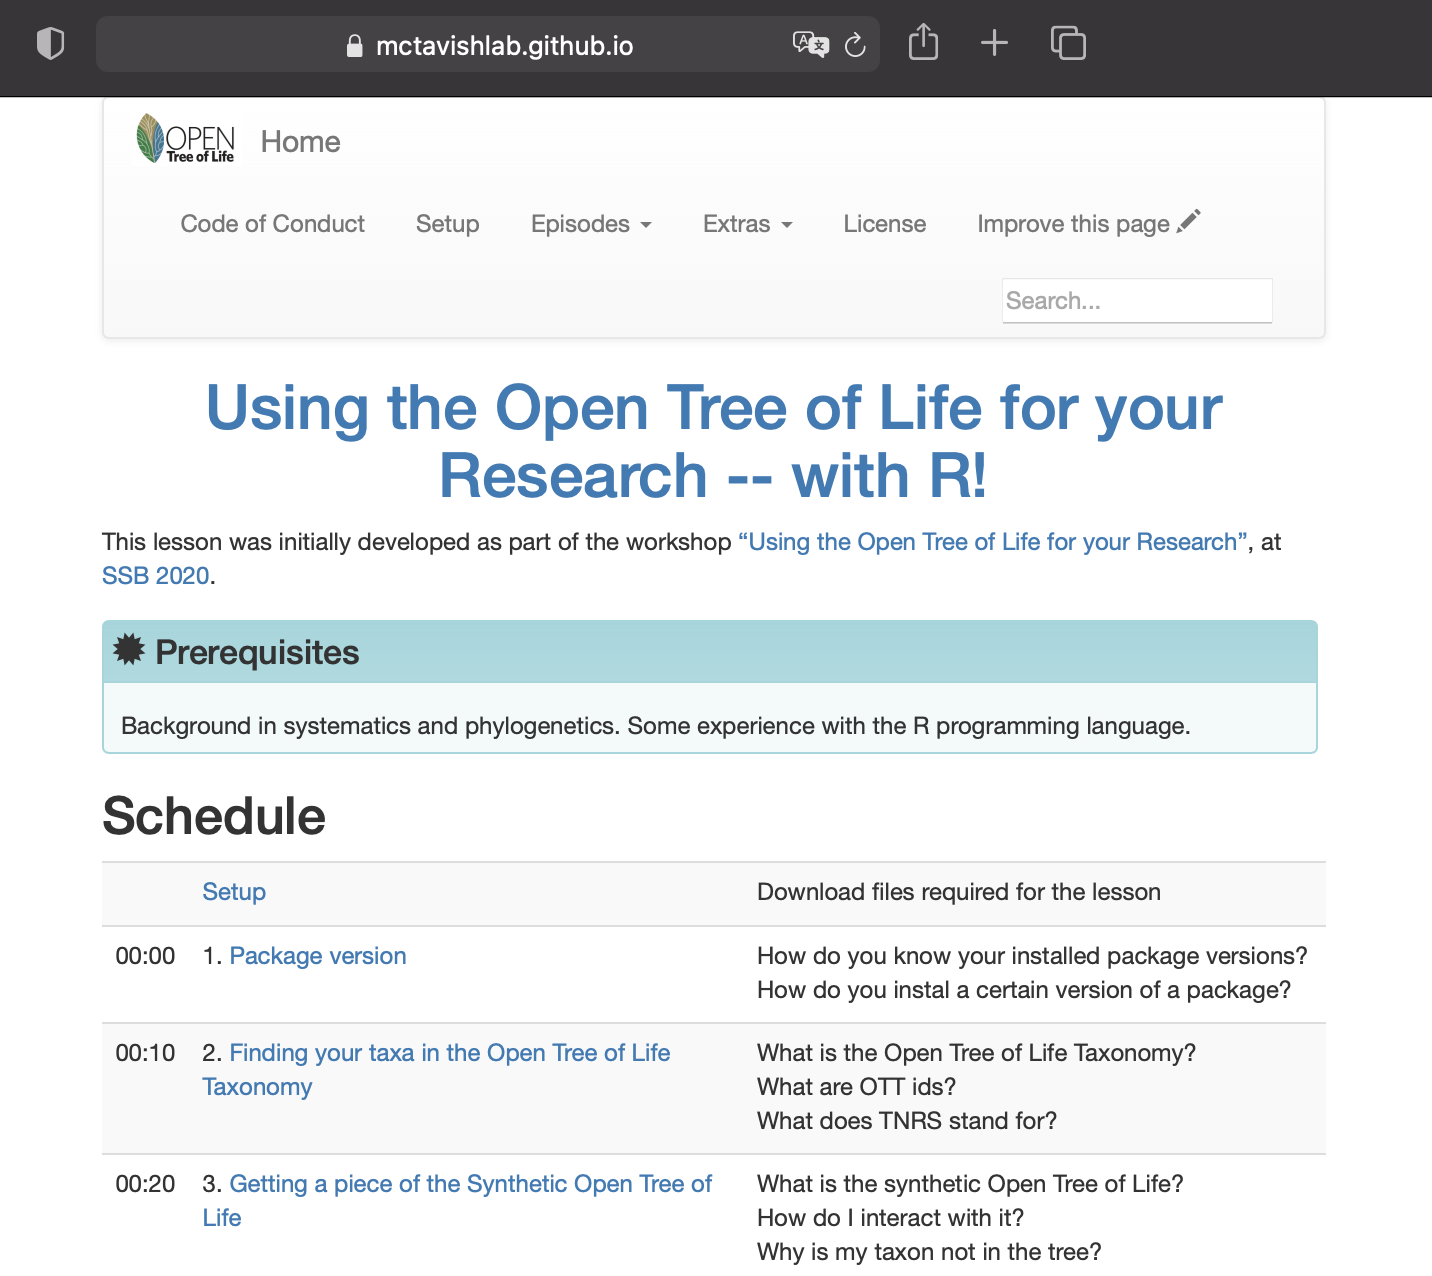
\includegraphics[width=3in]{fig-schedule.png}
\end{center}
\caption{Snapshot of the home to our tutorial website, showing part of the schedule. \label{fig:schedule}}
\end{figure}

We created a main version of the tutorial that is stable. Any updates to the tutorial are
published as new versions, or tutorials for new workshops \citep{wilson2006swc, SWCwebsite}
 Versions presented at workshops are a copy from the original repository.
They represent a temporally stable snapshot of functions and workflows presented
during a workshop.

%%% \subsubsection*{5. The (now) classics of computational reproducibility}
%%%
%%% Provide all information on package version and system capabilities.
%%%
%%% > [name=Emily Jane McTavish]link to where/and how you did that

\section*{Conclusion}
\label{sec:conclusion}

Response form the community has been invaluable in gauging success of the tutorials.
Senior researchers often comment on the usefulness
of the tutorials for their research, as well as supporting students in using the
R packages with less help from them as PIs.

Making accessible reproducible workflows has several advantages:

- save explanation/training time when analyses are run again by students and collaborators;
- save research time for yourself when analyses are run again with more data, a
  different dataset, a different organism or biological model;
- scientific efforts can build off of each other.


Ultimately, the long term improvement of reproducibility rates in science will depend
on our ability to intentionally integrate the subject of reproducibility into the
undergraduate curriculum, so college learners and future researchers have the
basis to develop the fundamental skills needed to successfully create reproducible
scientific workflows and materials.

Some universities have been incorporating the subject in their classes (see
\cite{uwlibraries2022, nigms2022}).
The focus of these resources has been for students to develop skills to document their work.
The principles identified and outlined here can be used to set learning goals and
outcomes on new reproducibility syllabi.

The principles to create tutorials described here facilitate adoption of software
 and analysis workflows among researchers at different academic levels, from undergrads
  to established researchers.
It will also help close the gap between students that had access to computational
resources (and computational training) from an early age and students that did not.
Late access to computational resources and training can occur due to lack of
economic resources, often occurring in households from underrepresented communities
and minorities \citep{REFERENCE-NEEDED}.
It can also be due to gender-biased parental and community pressures,
in which male individuals are more often encouraged to perform activities related to computers,
while female individuals are discouraged \citep{REFERENCE-NEEDED}.
% How to balance software acceptance VS. adoption?
These principles can be used to improve not only reproducibility practices,
 but also software adoption in the natural sciences.
%% Discuss: why address accessibility and not other aspects of reproducibility?


\bigskip
\begin{center}
{\large\bf SUPPLEMENTARY MATERIAL}
\end{center}

\begin{description}

\item[Title:] Website and GitHub repository containing the complete teaching materials developed and demonstrated here.

\item[GitHub repository link:] \url{https://github.com/McTavishLab/R_OpenTree_tutorials}

\item[Website link:] \url{https://mctavishlab.github.io/R_OpenTree_tutorials}

\end{description}

\bibliography{Manuscript-bibliography}

\end{document}
